% 1997 年全国卷理科第 23 题：正方体 ABCD-A_1B_1C_1D_1
% E 是 BB_1 的中点，F 是 CD 的中点；仅保留 TikZ 矢量源。
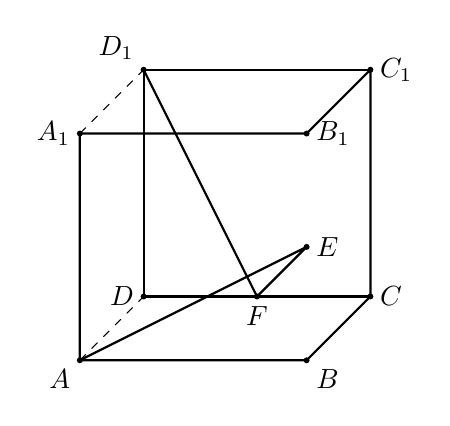
\begin{tikzpicture}[scale=0.9, >=stealth]
  \coordinate (A)  at (0,0);
  \coordinate (B)  at (3.2,0);
  \coordinate (C)  at (4.1,0.9);
  \coordinate (D)  at (0.9,0.9);
  \coordinate (A1) at (0,3.2);
  \coordinate (B1) at (3.2,3.2);
  \coordinate (C1) at (4.1,4.1);
  \coordinate (D1) at (0.9,4.1);
  \coordinate (E)  at (3.2,1.6);
  \coordinate (F)  at (2.5,0.9);

  \draw[thick] (A)--(B)--(C)--(C1)--(B1)--(A1)--cycle;
  \draw[thick] (D)--(C) (D)--(D1) (D1)--(C1);
  \draw[dashed] (A)--(D) (A1)--(D1);
  \draw[thick] (A)--(E) (E)--(F) (D1)--(F);

  \fill (A)  circle (1.2pt) node[below left] {$A$};
  \fill (B)  circle (1.2pt) node[below right] {$B$};
  \fill (C)  circle (1.2pt) node[right] {$C$};
  \fill (D)  circle (1.2pt) node[left] {$D$};
  \fill (A1) circle (1.2pt) node[left] {$A_1$};
  \fill (B1) circle (1.2pt) node[right] {$B_1$};
  \fill (C1) circle (1.2pt) node[right] {$C_1$};
  \fill (D1) circle (1.2pt) node[above left] {$D_1$};
  \fill (E)  circle (1.2pt) node[right] {$E$};
  \fill (F)  circle (1.2pt) node[below] {$F$};
\end{tikzpicture}
